\subsubsection{Index Finger Knuckle of Hand Dorsal Image Database}
\begin{figure}[H]
	\centering
	\begin{subfigure}[b]{0.8\linewidth}
		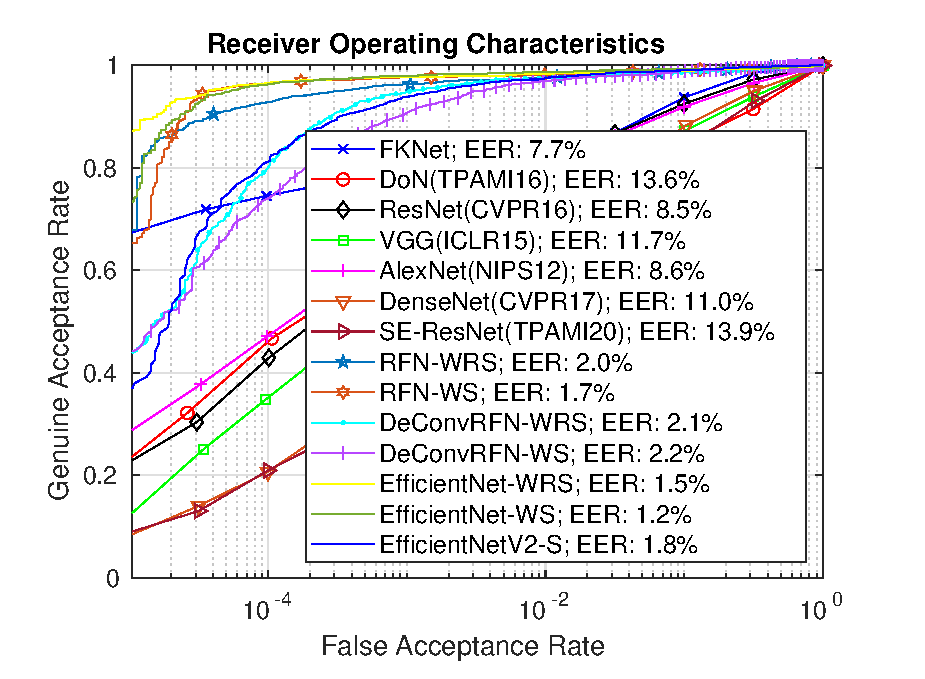
\includegraphics[width=\linewidth]{Figures/add-efficientv2-s/hd-roc_compare_new.eps}
	\end{subfigure}
	\begin{subfigure}[b]{0.8\linewidth}
		\includegraphics[width=\linewidth]{Figures/fknet/hd-cmc.eps}
	\end{subfigure}
\end{figure}

\textcolor{red}{For the ROC curve, I add EfficientNetV2-S model performance.} Update CMC Curve and ROC Curve with EfficientNet, DeConvRFNet and RFNet. As for the experiment, the dataset totally contains 712 subjects, and I use the segmented Index finger knuckle as my dataset. And I fine-tuned my model on the first sample of each subject, and then use the rest four sample as the testing dataset. At the testing process, it has $712*4=2848$ genuine matching scores, and has $712*711*4=2024928$ imposter matching scores. The performance of RFN-128-WRS and RFN-128-WS is similar, but the RFN-128-WS is slightly better than RFN-128-WRS depend on the EER value. And we can get an information that the RFNet is better than the rest network in the ROC figure, including the FKNet.